% Intended LaTeX compiler: pdflatex
\documentclass[10pt,article]{article}
\usepackage[utf8]{inputenc}
\usepackage[T1]{fontenc}
\usepackage{graphicx}
\usepackage{grffile}
\usepackage{longtable}
\usepackage{wrapfig}
\usepackage{rotating}
\usepackage[normalem]{ulem}
\usepackage{amsmath}
\usepackage{textcomp}
\usepackage{amssymb}
\usepackage{capt-of}
\usepackage{hyperref}
\usepackage{titling} \posttitle{\par\end{center}} \setlength{\droptitle}{-30pt} \usepackage{multicol} \setlength{\columnsep}{1cm} \usepackage[T1]{fontenc} \usepackage[utf8]{inputenc} \renewcommand{\contentsname}{Table of Contents / Agenda} \usepackage[letterpaper,left=1in,right=1in,top=0.7in,bottom=1in,headheight=23pt,includehead,includefoot,heightrounded]{geometry} \usepackage{fancyhdr} \pagestyle{fancy} \fancyhf{} \cfoot{\thepage} \usepackage{mathpazo} \usepackage[scaled=0.85]{helvet} \usepackage{courier} \usepackage[onehalfspacing]{setspace} \usepackage[framemethod=default]{mdframed} \usepackage{wrapfig} \usepackage{booktabs} \usepackage[outputdir=Lectures]{minted}
\setcounter{secnumdepth}{3}
\date{\vspace{-6ex}}
\title{Class 5: Design of Price and Advertising Elasticity Models}
\hypersetup{
 pdfauthor={},
 pdftitle={Class 5: Design of Price and Advertising Elasticity Models},
 pdfkeywords={},
 pdfsubject={Description School specific teaching materials},
 pdfcreator={Emacs 26.1 (Org mode 9.1.13)}, 
 pdflang={English}}
\begin{document}

\maketitle
\lhead{ COURSE 0000 \\ Joon H. Ro } 
\rhead{ Class 5 \\ 2018-09-11 Tue} 
\thispagestyle{fancy}

\setcounter{tocdepth}{1}
\tableofcontents
\vspace{6ex}

\section{Variable Transformations and Non-linear Effects}
\label{sec:orgf26ce2b}
\subsection{Previous Sales Model}
\label{sec:org230afc3}
\[ Sales = \beta_0 + \beta_1 \times Price + \beta_2 \times Advertising +
           \beta_3 \times Display \]

e.g., \(Sales = 100 -100 \times Price + 50 \times Advertising +
           1000 \times Display\)
\begin{itemize}
\item Is this an adequate model of the sales marketing mix relationship?
\end{itemize}

\iffalse
\[ Sales = \beta_0 + \beta_1 \times Price + \beta_2 \times Advertising +
           \beta_3 \times Display \]
\fi

\begin{itemize}
\item Problematic Implications: 
\begin{itemize}
\item Increasing advertising leads to consistent increase in sales
\item Increase in sales from a unit increase in advertising is same at all
levels of advertising
\item A price decrease always lead to an increase in sales
\begin{itemize}
\item Saturation point
\end{itemize}
\end{itemize}
\end{itemize}

\begin{itemize}
\item Solution: log transformation
\end{itemize}
\subsection{Log Transformation}
\label{sec:org7ea89a8}
\[ Sales = \beta_0 + \beta_1 \times \ln(Price) + \beta_2 \times
           \ln(Advertising) + \beta_3 \times Display \]
In general, two reasons to take a log:

\begin{enumerate}
\item A non-linear relationship (decreasing marginal return) exists between the
independent and dependent variables.
\end{enumerate}

\begin{center}
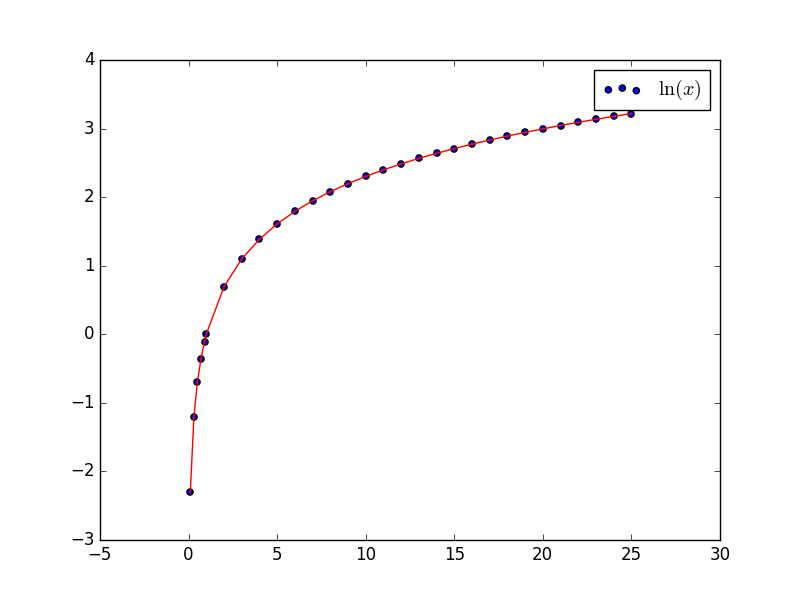
\includegraphics[width=8cm]{c:/Users/joon/Sync/Org-Coursepack/Assets/Images/Regression/ln_x.png}
\end{center}

\begin{itemize}
\item Examples: distance, income, etc
\end{itemize}
\subsection{Non-Linear Effects: Inverted-U Relationship}
\label{sec:orgcabae6b}
\begin{itemize}
\item Likelihood of Purchasing Candy Bar = \(1.1 + 3 \times \text{Sweetness}\)

\begin{itemize}
\item So should we keep adding sugar?
\end{itemize}

\item You can add a squared term (\(x^{2}\) when you expect inverted-U relationship
\end{itemize}

For example, if our results are:

\[ y = 1 + 3 \times x - 0.2 \times x^2 \]

the predicted \(y\) values (\(\hat y\)) are:

\begin{center}
\begin{tabular}{lrrrrrrrrrrrr}
\(x\) & 1 & 2 & 3 & 4 & 5 & 6 & 7 & 8 & 9 & 10 & 11 & 12\\
\(\hat y\) & 3.8 & 6.2 & 8.2 & 9.8 & 11 & 11.8 & 12.2 & 12.2 & 11.8 & 11.0 & 9.8 & 8.2\\
\end{tabular}
\end{center}
\section{Elasticities}
\label{sec:orgdca80a3}
\begin{itemize}
\item The measurement of how responsive an variable is to a change in another

\item The \(x\) (price, advertising, etc) elasticity of \(y\) (usually
demand or supply) is:

\[ \dfrac{\text{Percentage change in } y}{\text{Percentage change in } x} \]

\begin{itemize}
\item where

\[ \text{Percentage change in } x= \dfrac{\Delta x}{x} \]

where \(\Delta\) denotes the change
\end{itemize}
\end{itemize}
\subsection{Price Elasticity of Demand}
\label{sec:org8449561}
\begin{center}
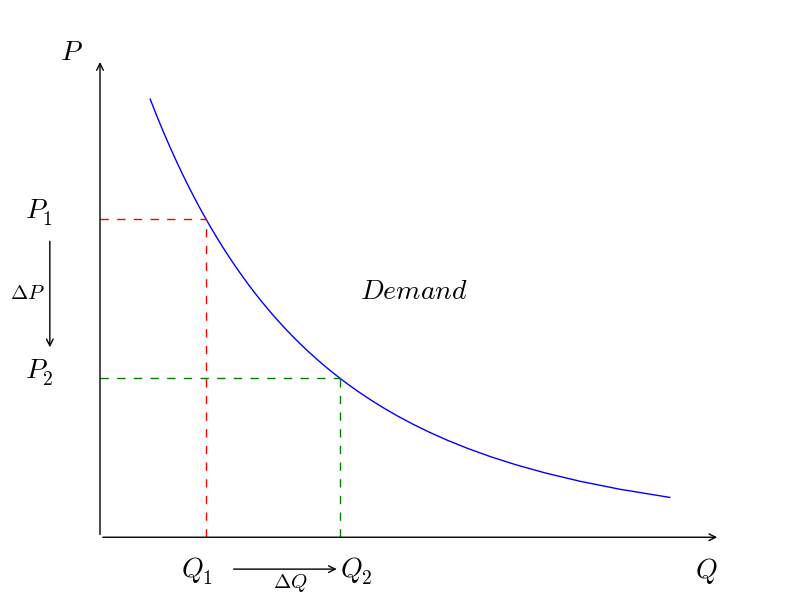
\includegraphics[width=8cm]{c:/Users/joon/Sync/Org-Coursepack/Assets/Images/Regression/Price_elasticity_of_demand.png}
\end{center}

\begin{itemize}
\item Price elasticity of demand (PED): 
\begin{itemize}
\item Percentage change in quantity demanded in response to a \textbf{1\% change} in
price (holding constant all the other marketing mix variables)
\end{itemize}
\end{itemize}

\begin{align*}
   PED & = \left\lvert \dfrac{\% \text{Changes in Sales (Quantity Demanded)}}{\% \text{Changes in Own Price}} \right\rvert \\
       & = \left\lvert \dfrac {\Delta Q}{Q} \Bigg/ \dfrac {\Delta P}{P} \right\rvert   \\
\end{align*}

\begin{center}
\begin{tabular}{lll}
Suppose Price increases 1\%, and demand is \((P)\) & Sales Decrease \((Q)\) & Total Revenue \(P \times Q\)\\
\hline
 Elastic (\( PED > 1 \)) &  More than 1 \% &  \( \Downarrow \)\\
 Unit Elastic (\( PED = 1 \)) &  1 \% &  \( \Longleftrightarrow \)\\
 Inelastic (\( PED < 1 \)) &  Less than 1 \% &  \( \Uparrow \)\\
\end{tabular}
\end{center}

\begin{mdframed}[frametitle={Note}]
Note that PED only looks at the size of the change because the direction of
the change is assumed to be negative.
\end{mdframed}

\subsubsection{Elasticities in Regression}
\label{sec:orgfa1da13}
\begin{itemize}
\item With a sample of historical data, you can measure the elasticities with the
log-log model:

\[ \ln(Q) = \beta_0 + \beta_1 \ln(P) + \varepsilon \]

\item (The size of) \(\beta_1\) represents the price elasticities of demand

\[ \ln(Q) = 10 -1.5 \ln(P) \]
\end{itemize}

\iffalse
\begin{itemize}
\item Derivation on the class notes
\end{itemize}
\fi

\begin{mdframed}[frametitle={Why?}]
Remember the interpretation of \(\beta\), the
coefficient of in linear regression is:

\[ 
   \dfrac{d Q}{d P} = \dfrac{d (\beta_0 + \beta_1 P +
   \varepsilon) }{d P} = \beta_1
\]

That is, the increase in \(Q\)  when \(P\)  increases by 1 unit

When you have a log-log model:

\[ \ln(Q) = \beta_0 + \beta_1 \ln (P) + \varepsilon\]

\[ \Rightarrow Q = \exp(\beta_0 + \beta_1 \ln (P) + \varepsilon ) \]

\[ \dfrac{d Q}{d P}  \quad = \underbrace{\exp(\beta_0 + \beta_1 \ln(P) +
          \varepsilon )}_{Q}
         \cdot \underbrace{\beta_1 \cdot \dfrac{1}{P}}_{\text{Chain Rule}} \\
           \quad =  Q \cdot \beta_1 \cdot \dfrac{1}{P} 
\]

\iffalse
\[    \dfrac{d Q}{d P}  = Q \cdot \beta_1 \cdot \dfrac{1}{P} \]
\fi

Hence,

\[       \beta_1 \quad = \dfrac{d Q}{Q} \cdot \dfrac{P}{d P} \\
                 \quad = \dfrac{d Q}{Q} \Bigg/ \dfrac{d P}{P} \]


NOTE: This derivation will not be on the exam
\end{mdframed}
\subsection{Cross Price Elasticities}
\label{sec:org6d69206}
\begin{itemize}
\item Elasticity between variables of two different products

\item Important because many products are \textbf{complements} or \textbf{substitutes} to each
other:

\begin{itemize}
\item Cannibalization
\end{itemize}
\end{itemize}

\begin{itemize}
\item Product 1's cross-price elasticity of product 2 would be:

\begin{itemize}
\item The impact of product 2's percentage change in prices on the percentage
change in product 1's sales
\end{itemize}
\end{itemize}

\[ \dfrac{\text{Changes in Sales (Quantity Demanded)}}{\text{Changes in
Price of Another Good}} = \dfrac{\Delta Q}{Q} \Bigg/ \dfrac{\Delta
P_{other}}{P_{other}} = \dfrac{d \ln (Q)}{d \ln (P_{other})} \]
\subsubsection{Cross Price Elasticities in Regression}
\label{sec:org81b7963}
\begin{itemize}
\item Hence, if you have the following model:

\[ \ln(Q) = \beta_0 + \beta_1\ln(P) + \beta_2\ln(P_{other}) + \varepsilon \]

\(\beta_{2}\) reflects the cross price elasticity
\end{itemize}

\begin{itemize}
\item If \(\beta_2\) is positive \ldots{}
\begin{itemize}
\item Other good price increases, your sales  increase 
 \( P_{other} \uparrow (Q_{other} \downarrow) \)  \(\Rightarrow Q\;\uparrow \)
\item e.g. Raise price of salsa and sales of cheese dip increase
\item Two products are \emph{substitute}
\end{itemize}
\end{itemize}

\begin{itemize}
\item If \(\beta_2\) is negative \ldots{}
\begin{itemize}
\item Other good price increases, your sales  decrease
 \( P_{other} \uparrow (Q_{other} \downarrow) \)  \( \Rightarrow Q\;\downarrow \)
\item e.g. Raise price of salsa and sales of chips decrease
\item Two products are \emph{complements}
\end{itemize}
\end{itemize}

\begin{itemize}
\item If \(\beta_2\) is zero (insignificant) \ldots{}
\begin{itemize}
\item Other good price increases, your sales  don't change
\item e.g. Raise price of salsa and sales of pasta sauce not affected
\item Two products are \emph{independent}
\end{itemize}
\end{itemize}
\subsection{The log-log sales response model}
\label{sec:org7dd24dc}
\iffalse
\begin{align*}
\ln(\text{sales in period } t) = \beta_0 + \beta_1 & \times \ln(\text{own
price in period } t) \\
                + \beta_2 & \times \ln(\text{competitor price in period } t)  + \varepsilon_t
\end{align*}
\fi

\[ \ln(\text{sales in period } t) = \beta_0 + \beta_1 \times \ln(\text{own
    price in period} t) + 
   \beta_2 \times \ln(\text{competitor price in period } t)  + \varepsilon_t
\]
\begin{itemize}
\item This model typically fits the data much better than the linear model
\item Coefficients to log(prices) may be interpreted as price elasticities
\end{itemize}
\subsection{Advertising Elasticity of Demand (AED)}
\label{sec:orgf844fc8}

\begin{itemize}
\item Just like the price elasticities of demand,
\item A measure to show the responsiveness of the quantity demanded of a good (or
service) to a change in the level of advertising:
\end{itemize}

\begin{align*}
  AED  & = \dfrac{\% \text{Changes in Sales}}{\% \text{Changes in Advertising}} \\
        & = \dfrac {\Delta Q}{Q} \Bigg/ \dfrac {\Delta A}{A}  \\
\end{align*}
\subsubsection{AED Regression}
\label{sec:org8b3a096}
Similarly, \(\beta_1\) in the following regression equation represents
the advertising elasticities of demand:

\[  \ln(Q) =  \beta_0 + \beta_1 \cdot \ln(A) + \varepsilon \]
\subsection{Price and Advertising Elasticity Model}
\label{sec:orgd4dd1e2}
You can estimate all the elasticities with the following model:

\begin{align*}
\ln(\text{Sales in period } t) = \beta_0 + \beta_{own} & \times \ln(\text{Own Price in period } t) \\
                                         + \beta_{cross} & \times \ln(\text{Other Good Price in period } t) \\
                                         + \beta_{ad} & \times \ln (\text{Advertising}_t) \\
                                         + \beta_{display} & \times \text{Display}_t
\end{align*}
\iffalse
\begin{align*}
\ln(\text{Sales in period } t) = \beta_0 + \beta_{own} & \times \ln(\text{Own Price in period } t) \\
                                         + \beta_{cross} & \times \ln(\text{Other Good Price in period } t) \\
                                         + \beta_{ad} & \times \ln (\text{Advertising}_t) \\
                                         + \beta_{display} & \times \text{Display}_t
\end{align*}
\fi

\begin{itemize}
\item Interpretation of Coefficients:
\begin{itemize}
\item \(\beta_{own}\): own price elasticity
\item \(\beta_{cross}\): cross price elasticity
\item \(\beta_{ad}\): advertising elasticity
\item \(\beta_{display}\): impact of display on sales
\end{itemize}
\end{itemize}

\begin{mdframed}[frametitle={Interpretation of \( \beta_{display} \)}]
The Display dummy equals to 1 when the product is on display. Hence, \(\beta_{display}\) represents the increase in \(\ln(\text{Sales})\) when the
product is on display comparing to the baseline case where the product is not
on display.  That is,

\[ \beta_{display} = \ln(\text{Sales}_{Display}) - \ln(\text{Sales}_{NoDisplay}) \]
\[ \Rightarrow \beta_{display} = \ln\left(\dfrac{\text{Sales}_{Display}}{\text{Sales}_{NoDisplay}}\right) \]
\[ \Rightarrow \exp(\beta_{display}) = \dfrac{\text{Sales}_{Display}}{\text{Sales}_{NoDisplay}} \]

Hence, \(\exp(\beta_{display})\) is the ratio between the two sales. For
example, if \(\beta_{display}\) were 0.3, \(\exp(0.3) = 1.35\), which
means a product's sales increase by 35\% when it is on display compared to when
it is not.
\end{mdframed}
\end{document}